\documentclass[12pt,a4paper]{article}

%\usepackage[utf-8]{inputenc}
\usepackage[margin=1in]{geometry}
\usepackage{graphicx}
\usepackage{hyperref}
\usepackage{xcolor}
\usepackage{fancyhdr}
\usepackage{tocloft}
\usepackage{float}
\usepackage{tabularx}
\usepackage{listings}

% ---------- Listing style (NO line-number column) ----------
\definecolor{codegray}{rgb}{0.5,0.5,0.5}
\definecolor{codepurple}{rgb}{0.58,0,0.82}
\definecolor{backcolour}{rgb}{0.95,0.95,0.92}

\lstdefinestyle{mystyle}{
  backgroundcolor=\color{backcolour},
  commentstyle=\color{codegray},
  keywordstyle=\color{codepurple},
  basicstyle=\ttfamily\small,
  breakatwhitespace=false,
  breaklines=true,
  captionpos=b,
  keepspaces=true,
  numbers=none,              % <-- removes the left index area completely
  numbersep=0pt,
  showspaces=false,
  showstringspaces=false,
  showtabs=false,
  tabsize=2
}
\lstset{style=mystyle}

\pagestyle{fancy}
\fancyhf{}
\rhead{ESP32 IoT Home Automation}
\lhead{Complete Implementation Guide}
\cfoot{\thepage}

\title{\textbf{ESP32 Arduino IoT Cloud} \\ \textbf{Home Automation System} \\ Complete Setup \& Implementation Guide}
\author{IoT Project Documentation}
\date{December 2025}

\begin{document}

\maketitle
\newpage
\tableofcontents
\newpage

% =========================================================
\section{Introduction}

We created a smart home automation system using an ESP32 microcontroller that controls lights and fans both \textbf{manually} (wall switches) and \textbf{remotely} (Arduino IoT Cloud dashboard). This version of the firmware uses a temporary hardcoded Wi-Fi SSID/password, but the system logic (local control + cloud sync + Eco mode + sensing) stays the same.

The system includes automatic motion-based control (Eco mode) and environmental monitoring (temperature and humidity) using a DHT11 sensor read via the \texttt{DHTesp} library.

% =========================================================
\newpage
\section{Part 1: What We Built (Project Overview)}

\subsection{The Goal}

We wanted to create a device that:

\begin{enumerate}
\item Controls \textbf{Light} and \textbf{Fan} relays via wall switches (always works, even offline)
\item Allows remote control via \textbf{Arduino IoT Cloud and Arduino Iot Android App and Google Home with Google Assistant Voice Command} (when Wi-Fi is available)
\item Automatically turns off outputs when \textbf{no motion} is detected (Eco mode)
\item Measures and reports \textbf{temperature and humidity} to the cloud
\item Connects to Wi-Fi using hardcoded SSID and password inside the sketch
\end{enumerate}

\subsection{Why We Chose Each Component}

\subsubsection{ESP32 Microcontroller}
\begin{itemize}
\item Affordable and powerful
\item Built-in Wi-Fi and Bluetooth
\item Enough GPIO pins for relays, switches, and sensors
\item Can be powered from a simple USB charger
\end{itemize}

\subsubsection{4-Channel Relay Module (active-LOW)}
\begin{itemize}
\item Safely switches AC mains voltage (Light and Fan sockets)
\item Isolates the low-voltage ESP32 from dangerous AC current
\item ``Active-LOW'' means GPIO outputs LOW to turn relay ON (HIGH to turn OFF)
\item We used 2 channel but can add and expand.
\end{itemize}

\subsubsection{DHT11 Temperature \& Humidity Sensor}
\begin{itemize}
\item Affordable environmental sensor
\item Provides both temperature (°C) and humidity (\%)
\item Temperature Range: 0° to 50°
\item Humidity Range: 20\% to 90\%
\item 
\item Operating Voltage: 5V
\item Used with \texttt{DHTesp} library for ESP32-friendly readings
\end{itemize}

\subsubsection{HC-SR501 PIR Motion Sensor}
\begin{itemize}
\item Detects human motion
\item Used for Eco mode (auto turn-off after no motion for 5 minutes)
\item Works as a simple digital output: HIGH when motion detected
\end{itemize}

\subsubsection{Wall Switches}
\begin{itemize}
\item Standard momentary switches wired to GND
\item Provide manual override regardless of cloud status
\end{itemize}

% =========================================================
\newpage
\section{Part 2: Hardware Setup}

\subsection{Wiring Schematic}

We used the following circuit connections:

\begin{figure}[H]
\centering
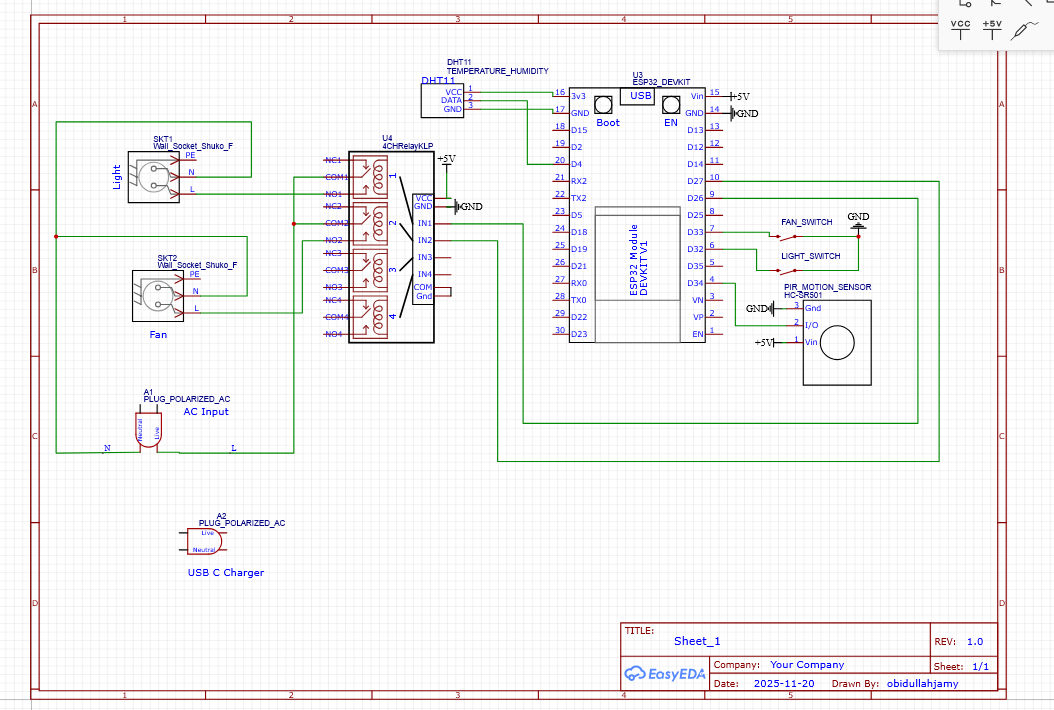
\includegraphics[width=0.95\textwidth]{circuit_diagram.jpg}
\caption{ESP32 Home Automation Circuit Diagram showing AC input (A1), USB power (A2), relay module, switches, PIR sensor, and DHT11 sensor connections}
\label{fig:schematic}
\end{figure}

\subsection{Key Connection Points}

\begin{table}[H]
\centering
\begin{tabularx}{\textwidth}{|l|l|X|}
\hline
\textbf{Component} & \textbf{ESP32 Pin} & \textbf{Purpose} \\
\hline
Relay Light (IN) & GPIO26 & Controls the Light relay (active-LOW) \\
\hline
Relay Fan (IN) & GPIO27 & Controls the Fan relay (active-LOW) \\
\hline
Light Switch & GPIO33 & Wall switch input (pressed = GND) \\
\hline
Fan Switch & GPIO32 & Wall switch input (pressed = GND) \\
\hline
PIR Motion Sensor & GPIO34 & Motion detection (HIGH = motion) \\
\hline
DHT11 Data & GPIO4 & Temperature/humidity sensor data \\
\hline
GND & GND & All grounds connected together \\
\hline
+5V & 5V (USB) & Powers relay, PIR, and DHT11 \\
\hline
\end{tabularx}
\caption{ESP32 Pin Connections}
\label{tab:pins}
\end{table}

\subsection{Power Supply}
\begin{itemize}
\item The ESP32 is powered via a \textbf{USB charger (A2 in the diagram)}
\item The \textbf{5V output} from the USB connection powers the relay module, PIR sensor, and DHT11
\item All ground pins are connected together
\end{itemize}

\subsection{Why These Specific Pins?}
GPIO34 is input-only, making it a good choice for the PIR sensor input. GPIO32 and GPIO33 work well with \texttt{INPUT\_PULLUP} for switches. GPIO26 and GPIO27 are standard output GPIO pins suitable for relay control.

% =========================================================
\newpage
\section{Part 3: Software Setup}

\subsection{Replicate the Steps (Cloud Setup)}

\subsubsection{Step 1: Go to Arduino IoT Cloud Website}
Open the Arduino IoT Cloud dashboard: \url{https://create.arduino.cc/iot/things}.

\subsubsection{Step 2: Create a Device}
\begin{itemize}
\item In Arduino IoT Cloud, create/select an ESP32 device.
\item Download the ``Device configuration'' PDF to get \textbf{DEVICE\_ID} and \textbf{DEVICE\_KEY}.
\end{itemize}

\subsubsection{Step 3: Create a Thing}
Create a new ``Thing'' and attach the device you created.

\subsubsection{Step 4: Create the Variables (must match code)}
Create these 5 variables in the Thing (names must match exactly):

\begin{enumerate}
\item \textbf{light} (Boolean) - Read/Write
\item \textbf{fan} (Boolean) - Read/Write
\item \textbf{eco} (Boolean) - Read/Write
\item \textbf{temperature} (Float) - Read only
\item \textbf{humidity} (Float) - Read only
\end{enumerate}

\subsubsection{Step 5: Create Dashboard Widgets}
\begin{itemize}
\item 3 Toggle switches (light, fan, eco)
\item 2 Value display widgets (temperature, humidity)
\end{itemize}

\subsection{Required Libraries (Arduino IDE)}

Install these from Arduino IDE Library Manager:

\begin{itemize}
\item \textbf{ArduinoIoTCloud}
\item \textbf{Arduino\_ConnectionHandler}
\item \textbf{DHTesp} (for DHT11 on ESP32)
\end{itemize}

Note: This firmware version does \textbf{not} use WiFiManager or a captive portal; Wi-Fi credentials are temporarily hardcoded in the sketch.

\subsection{Google Home / Google Assistant Integration}

\begin{itemize}
\item Enable ``Google Assistant Integration'' in the Arduino IoT Cloud Thing settings, then link your Arduino account inside the Google Home app.
\item Voice control typically works for \textbf{light}, \textbf{fan}, and \textbf{eco} because they are switch-like properties.
\item \textbf{temperature} is Read Only, but it can be queried by voice (read/report) depending on Google Home behavior and how Arduino Cloud exposes the sensor.
\item \textbf{humidity} is not supported for voice reporting in your setup (as requested).
\end{itemize}

% =========================================================
\newpage
\section{Part 4: The Code Explained (Block by Block)}

This section explains the firmware in logical blocks (matching the structure of your sketch).

\subsection{Block 1: Credentials (Cloud + Wi-Fi)}
\begin{itemize}
\item \texttt{DEVICE\_ID} and \texttt{DEVICE\_KEY} authenticate the device to Arduino IoT Cloud.
\item \texttt{WIFI\_SSID} and \texttt{WIFI\_PASS} are temporarily hardcoded Wi-Fi credentials (easy for testing).
\end{itemize}

\subsection{Block 2: Includes (Libraries)}
\begin{itemize}
\item \texttt{ArduinoIoTCloud.h} and \texttt{Arduino\_ConnectionHandler.h} handle Arduino IoT Cloud connectivity and syncing variables.
\item \texttt{WiFi.h} is the ESP32 Wi-Fi stack.
\item \texttt{Preferences.h} stores states (Light/Fan/Eco) in flash so they survive power loss.
\item \texttt{DHTesp.h} reads the DHT11 on ESP32 and provides a combined temperature+humidity read.
\end{itemize}

\subsection{Block 3: Pin Definitions}
All GPIO pins are defined once at the top so wiring changes are easy to apply.

\subsection{Block 4: Cloud Variables}
\begin{itemize}
\item \texttt{light}, \texttt{fan}, \texttt{eco} are booleans synchronized with the cloud (Read/Write).
\item \texttt{temperature}, \texttt{humidity} are floats synchronized to cloud as Read Only values.
\item They start at 0.0f (instead of \texttt{NAN}) to avoid dashboards showing blank values before the first reading.
\end{itemize}

\subsection{Block 5: Preferences Keys (Flash Storage)}
\begin{itemize}
\item Namespace \texttt{homeauto} groups saved values.
\item Keys \texttt{L}, \texttt{F}, \texttt{ECO} store relay and eco states.
\end{itemize}

\subsection{Block 6: Sensor + Timing}
\begin{itemize}
\item \texttt{DHTesp dht;} manages the DHT11.
\item \texttt{ECO\_OFF\_TIME} is 5 minutes.
\item \texttt{DHT\_PERIOD} is 5 seconds (DHT11 should not be read too frequently).
\end{itemize}

\subsection{Block 7: Cloud Callbacks}
When the cloud changes \texttt{light}, \texttt{fan}, or \texttt{eco}, the callback stores the new value in flash. The variable \texttt{ignoreCloudUntil} prevents immediate overwrite during reconnect.

\subsection{Block 8: initProperties()}
This registers each variable with Arduino IoT Cloud and sets permissions:
\begin{itemize}
\item Light/Fan/Eco: Read/Write, with callbacks
\item Temperature/Humidity: Read Only (device publishes)
\end{itemize}

\subsection{Block 9: Relay Output Function}
\texttt{applyRelays()} applies the final output state to active-LOW relays and also respects Eco mode by using the \texttt{allowOn} flag.

\subsection{Block 10: Wi-Fi + Cloud Start}
\begin{itemize}
\item \texttt{connectWiFi()} connects using \texttt{wifiSsid} / \texttt{wifiPass}.
\item \texttt{startCloud()} creates a \texttt{WiFiConnectionHandler} and begins Arduino Cloud updates.
\end{itemize}

\subsection{Block 11: setup()}
\begin{itemize}
\item Configures pins, initializes DHT11, loads saved relay states, registers cloud properties.
\item Copies hardcoded SSID/password into runtime buffers and connects Wi-Fi.
\end{itemize}

\subsection{Block 12: loop()}
\begin{itemize}
\item Updates Arduino Cloud (if started).
\item Reads PIR sensor and applies Eco logic.
\item Reads wall switches and saves state changes.
\item Reads DHT11 every 5 seconds and updates cloud variables.
\item Updates relays continuously.
\end{itemize}

% =========================================================
\newpage
\section{Part 5: Algorithm \& Flow Diagram}

\subsection{How the System Works}

\begin{figure}[H]
\centering
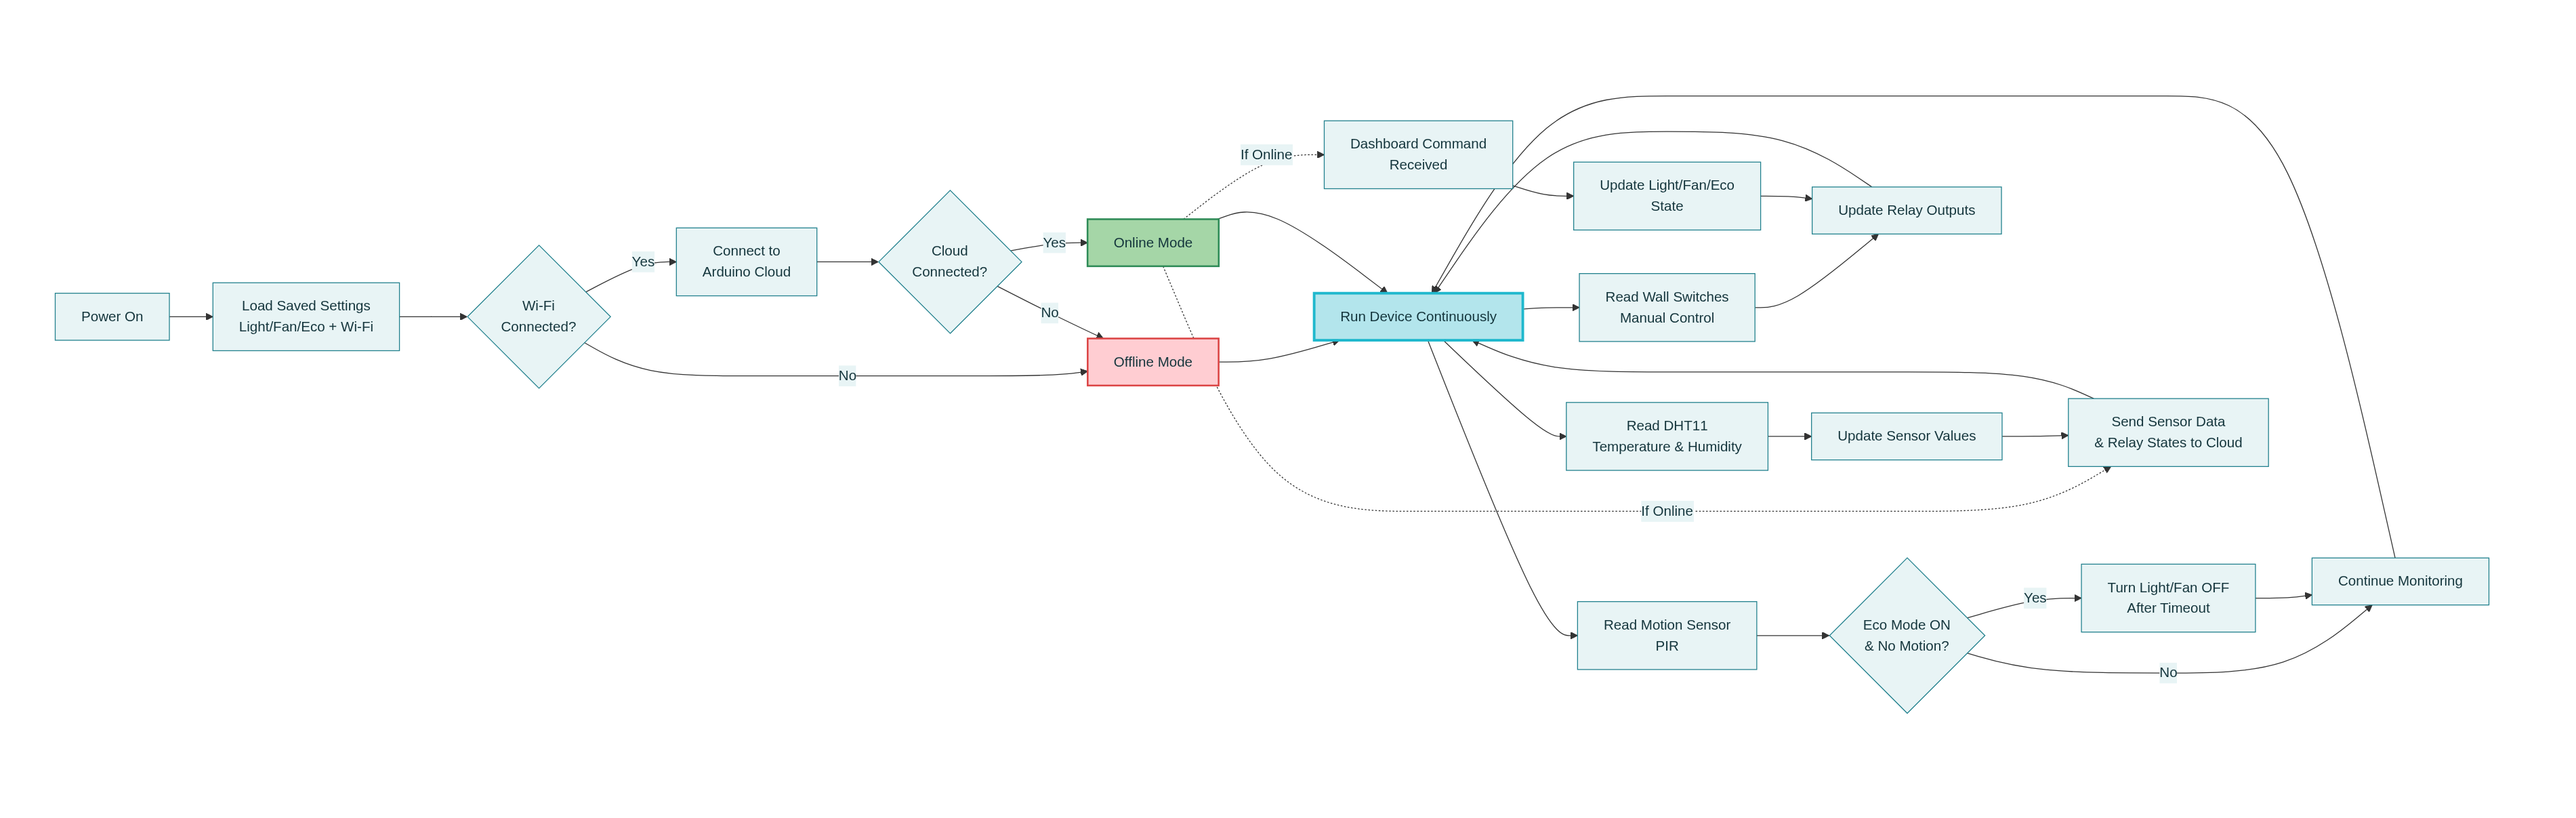
\includegraphics[width=0.95\textwidth]{flowchart.png}
\caption{System Flowchart: Startup, Wi-Fi connection (hardcoded credentials in this version), local control loop, cloud sync, Eco logic, and sensor updates}
\label{fig:flowchart}
\end{figure}

\subsection{Detailed Logic Flow}

\subsubsection{Startup:}
\begin{enumerate}
\item Power on $\rightarrow$ load saved Light/Fan/Eco states from flash
\item Configure GPIO, start DHT sensor
\item Connect to Wi-Fi using hardcoded credentials (temporary)
\item If Wi-Fi succeeds $\rightarrow$ connect to Arduino IoT Cloud
\item If Wi-Fi fails $\rightarrow$ keep working offline with switches + Eco + sensors (cloud won’t update)
\end{enumerate}

\subsubsection{Main Loop:}
\begin{enumerate}
\item Update Arduino IoT Cloud connection (if enabled)
\item Read PIR and update last motion time
\item If Eco is ON and no motion for 5 minutes $\rightarrow$ outputs forced OFF
\item Read wall switches and update \texttt{light} / \texttt{fan}
\item Read DHT11 every 5 seconds and update \texttt{temperature} / \texttt{humidity}
\item Apply relay outputs (active-LOW)
\end{enumerate}

% =========================================================
\newpage
\section{Part 6: Complete Final Code}

\begin{lstlisting}[language=C++, caption=Complete ESP32 IoT Home Automation Code (Hardcoded Wi-Fi + DHTesp)]
/************  CHANGE ONLY THESE (from Arduino IoT Cloud PDF)  ************/
const char DEVICE_ID[]  = "b3fcdc65-ac5f-4c0e-9193-b642c288a35f";
const char DEVICE_KEY[] = "LEsyu9jKdWH7UVcwfHT@9yker";
/**************************************************************************/

/************  HARDCODED WIFI (temporary)  ************/
const char WIFI_SSID[] = "Heaven";
const char WIFI_PASS[] = "avatar@123A";   // "" for open Wi-Fi
/*****************************************************/

#include <ArduinoIoTCloud.h>
#include <Arduino_ConnectionHandler.h>
#include <WiFi.h>
#include <Preferences.h>
#include <DHTesp.h>  // DHTesp library (beegee-tokyo).

// ---------------- Pins (match your diagram) ----------------
const int RELAY_LIGHT_PIN  = 26;   // Relay IN for Light (active-LOW)
const int RELAY_FAN_PIN    = 27;   // Relay IN for Fan   (active-LOW)
const int SWITCH_FAN_PIN   = 32;   // FAN_SWITCH   -> GPIO32 -> to GND when pressed
const int SWITCH_LIGHT_PIN = 33;   // LIGHT_SWITCH -> GPIO33 -> to GND when pressed
const int PIR_PIN          = 34;   // PIR OUT -> GPIO34 (input-only pin)
const int DHT_PIN          = 4;    // DHT11 DATA -> D4 (GPIO4)
// -----------------------------------------------------------

// -------- Cloud variables (must match your Thing variable names) ------
bool  light = false;
bool  fan   = false;
bool  eco   = false;

// Don’t initialize with NAN (dashboards may show blank / no value)
float temperature = 0.0f;
float humidity    = 0.0f;
// ---------------------------------------------------------------------

// ---------------- Saved settings / state ----------------
Preferences prefs;

// Saved relay + eco state
const char* NS_APP = "homeauto";
const char* K_L    = "L";
const char* K_F    = "F";
const char* K_ECO  = "ECO";

// ---------------- Sensors ----------------
DHTesp dht;

// ---------------- Timings ----------------
unsigned long lastMotionTime = 0;
const unsigned long ECO_OFF_TIME = 5UL * 60UL * 1000UL;  // 5 minutes

unsigned long lastDhtRead = 0;
const unsigned long DHT_PERIOD = 5000;                  // 5 seconds (safe for DHT11)

// ---------------- Wi-Fi / Cloud runtime ----------------
char wifiSsid[33] = {0};
char wifiPass[65] = {0};

WiFiConnectionHandler* cloudConn = nullptr;
bool cloudStarted = false;

// Prevent “instant overwrite” when cloud reconnects
unsigned long ignoreCloudUntil = 0;

// ---------------- Wall switch edge detect ----------------
bool prevLightSw = false;
bool prevFanSw   = false;

// ---------- Cloud callbacks ----------
void onLightChange() {
  if (millis() < ignoreCloudUntil) return;
  prefs.putBool(K_L, light);
}

void onFanChange() {
  if (millis() < ignoreCloudUntil) return;
  prefs.putBool(K_F, fan);
}

void onEcoChange() {
  if (millis() < ignoreCloudUntil) return;
  if (eco) lastMotionTime = millis();
  prefs.putBool(K_ECO, eco);
}

// ---------- Cloud properties ----------
void initProperties() {
  ArduinoCloud.setBoardId(DEVICE_ID);
  ArduinoCloud.setSecretDeviceKey(DEVICE_KEY);

  ArduinoCloud.addProperty(light, READWRITE, ON_CHANGE, onLightChange);
  ArduinoCloud.addProperty(fan,   READWRITE, ON_CHANGE, onFanChange);
  ArduinoCloud.addProperty(eco,   READWRITE, ON_CHANGE, onEcoChange);

  ArduinoCloud.addProperty(temperature, READ, ON_CHANGE, NULL);
  ArduinoCloud.addProperty(humidity,    READ, ON_CHANGE, NULL);
}

// ---------- Helpers ----------
void applyRelays(bool allowOn) {
  bool outLight = allowOn && light;
  bool outFan   = allowOn && fan;

  // active-LOW relay
  digitalWrite(RELAY_LIGHT_PIN, outLight ? LOW : HIGH);
  digitalWrite(RELAY_FAN_PIN,   outFan   ? LOW : HIGH);
}

void loadSavedState() {
  light = prefs.getBool(K_L, false);
  fan   = prefs.getBool(K_F, false);
  eco   = prefs.getBool(K_ECO, false);
}

bool connectWiFi(unsigned long timeoutMs = 15000) {
  if (strlen(wifiSsid) == 0) return false;

  WiFi.mode(WIFI_STA);
  WiFi.begin(wifiSsid, wifiPass);

  unsigned long start = millis();
  while (WiFi.status() != WL_CONNECTED && (millis() - start) < timeoutMs) {
    delay(50);
  }
  return (WiFi.status() == WL_CONNECTED);
}

void startCloud() {
  if (cloudConn) {
    delete cloudConn;
    cloudConn = nullptr;
  }

  cloudConn = new WiFiConnectionHandler(wifiSsid, wifiPass);
  ArduinoCloud.begin(*cloudConn);
  cloudStarted = true;

  // After reconnect, push local values first for a moment
  ignoreCloudUntil = millis() + 2000;
}

void setup() {
  Serial.begin(115200);
  delay(500);

  // GPIO setup
  pinMode(RELAY_LIGHT_PIN, OUTPUT);
  pinMode(RELAY_FAN_PIN,   OUTPUT);
  digitalWrite(RELAY_LIGHT_PIN, HIGH); // off (active-LOW)
  digitalWrite(RELAY_FAN_PIN,   HIGH); // off (active-LOW)

  pinMode(SWITCH_LIGHT_PIN, INPUT_PULLUP);
  pinMode(SWITCH_FAN_PIN,   INPUT_PULLUP);
  pinMode(PIR_PIN,          INPUT);

  // DHTesp init for DHT11
  dht.setup(DHT_PIN, DHTesp::DHT11);

  // Load saved relay/eco state
  prefs.begin(NS_APP, false);
  loadSavedState();

  // Initialize edge detector baselines
  prevLightSw = (digitalRead(SWITCH_LIGHT_PIN) == LOW);
  prevFanSw   = (digitalRead(SWITCH_FAN_PIN)   == LOW);

  lastMotionTime = millis();
  applyRelays(true);

  // Cloud setup
  initProperties();

  // Hardcoded Wi-Fi credentials
  strlcpy(wifiSsid, WIFI_SSID, sizeof(wifiSsid));
  strlcpy(wifiPass, WIFI_PASS, sizeof(wifiPass));

  if (connectWiFi()) {
    startCloud();
  }

  Serial.print("WiFi: ");
  Serial.println((WiFi.status() == WL_CONNECTED) ? "connected" : "offline");
  Serial.print("IP: ");
  Serial.println(WiFi.localIP());
}

void loop() {
  // Keep the IoT Cloud connection alive (must be called frequently).
  if (cloudStarted) {
    ArduinoCloud.update();
  }

  // 1) Motion sensor (for Eco mode)
  if (digitalRead(PIR_PIN) == HIGH) lastMotionTime = millis();

  bool allowOn = true;
  if (eco) allowOn = (millis() - lastMotionTime < ECO_OFF_TIME);

  // 2) Wall switches (manual control)
  bool lightSw = (digitalRead(SWITCH_LIGHT_PIN) == LOW);
  bool fanSw   = (digitalRead(SWITCH_FAN_PIN)   == LOW);

  if (lightSw != prevLightSw) {
    prevLightSw = lightSw;
    light = lightSw;
    prefs.putBool(K_L, light);
  }

  if (fanSw != prevFanSw) {
    prevFanSw = fanSw;
    fan = fanSw;
    prefs.putBool(K_F, fan);
  }

  // 3) DHT11 sensor (periodic reading)
  if (millis() - lastDhtRead >= DHT_PERIOD) {
    lastDhtRead = millis();

    TempAndHumidity th = dht.getTempAndHumidity(); // Single call reads both
    if (!isnan(th.temperature) && !isnan(th.humidity)) {
      temperature = th.temperature;
      humidity    = th.humidity;
    }

    // Debug (optional)
    Serial.print("DHT -> H: ");
    Serial.print(th.humidity, 0);
    Serial.print("%  T: ");
    Serial.print(th.temperature, 0);
    Serial.print("C  Status: ");
    Serial.println(dht.getStatusString());
  }

  // 4) Update relays
  applyRelays(allowOn);

  delay(30);
}
\end{lstlisting}

% =========================================================
\newpage
\section{Part 7: How to Replicate This Project}

\subsection{Step 1: Arduino IoT Cloud Setup}
\begin{enumerate}
\item Go to \url{https://create.arduino.cc/iot/things}
\item Create a Device (ESP32) and download the Device Configuration PDF
\item Create a Thing and attach your Device
\item Create the variables exactly as in the code:
\begin{itemize}
\item \texttt{light} (Boolean, Read/Write)
\item \texttt{fan} (Boolean, Read/Write)
\item \texttt{eco} (Boolean, Read/Write)
\item \texttt{temperature} (Float, Read Only)
\item \texttt{humidity} (Float, Read Only)
\end{itemize}
\item Create a dashboard with 3 toggles and 2 value widgets
\end{enumerate}

\subsection{Step 2: Arduino IDE Setup (Libraries)}
\begin{enumerate}
\item Open Arduino IDE $\rightarrow$ Library Manager
\item Install: \texttt{ArduinoIoTCloud}, \texttt{Arduino\_ConnectionHandler}, \texttt{DHTesp}
\end{enumerate}

\subsection{Step 3: Configure Firmware}
\begin{enumerate}
\item Paste the code from Part 6 into a new sketch
\item Set your \textbf{DEVICE\_ID} and \textbf{DEVICE\_KEY} from the PDF
\item (Temporary) set \textbf{WIFI\_SSID} and \textbf{WIFI\_PASS} to your router credentials
\end{enumerate}

\subsection{Step 4: Upload and Test}
\begin{enumerate}
\item Select Tools $\rightarrow$ Board $\rightarrow$ ESP32 Dev Module
\item Select correct COM port
\item Upload
\item Test:
\begin{itemize}
\item Manual switches control relays
\item Dashboard toggles control relays when Wi-Fi is connected
\item Eco mode turns outputs off after 5 minutes of no motion
\item Temperature/humidity appear on dashboard
\end{itemize}
\end{enumerate}

\subsection{Step 5: Google Home Integration}
\begin{enumerate}
\item In Arduino IoT Cloud, enable ``Google Assistant Integration''
\item In Google Home app, link your Arduino account
\item Test voice:
\begin{itemize}
\item Turn on/off light
\item Turn on/off fan
\item Turn on/off eco
\item Ask temperature (read-only)
\item Humidity is not supported for voice (as requested)
\end{itemize}
\end{enumerate}

% =========================================================
\newpage
\section{Part 8: Troubleshooting}

\begin{table}[H]
\centering
\begin{tabularx}{\textwidth}{|l|X|}
\hline
\textbf{Problem} & \textbf{Solution} \\
\hline
Device won't connect to cloud & Check DEVICE\_ID and DEVICE\_KEY copied correctly from the IoT Cloud PDF. \\
\hline
Wi-Fi stays offline & Verify WIFI\_SSID / WIFI\_PASS in the code; confirm router password; check 2.4GHz Wi-Fi availability. \\
\hline
Relays don't switch & Check GPIO pins match wiring; confirm relay module is active-LOW (LOW = ON). \\
\hline
Wall switches don't work & Confirm switches go to GND and use \texttt{INPUT\_PULLUP}. \\
\hline
DHT11 values wrong or not updating & Check DHT wiring; ensure DHT11 selected in \texttt{dht.setup(..., DHTesp::DHT11)}; avoid reading faster than every 2 seconds (this code uses 5 seconds). \\
\hline
Eco mode doesn't turn off outputs & Check PIR sensor output and wiring; verify \texttt{eco} is ON in dashboard. \\
\hline
\end{tabularx}
\caption{Troubleshooting Guide}
\label{tab:troubleshooting}
\end{table}

% =========================================================
\newpage
\appendix
\section{Circuit Diagram}

\begin{figure}[H]
\centering
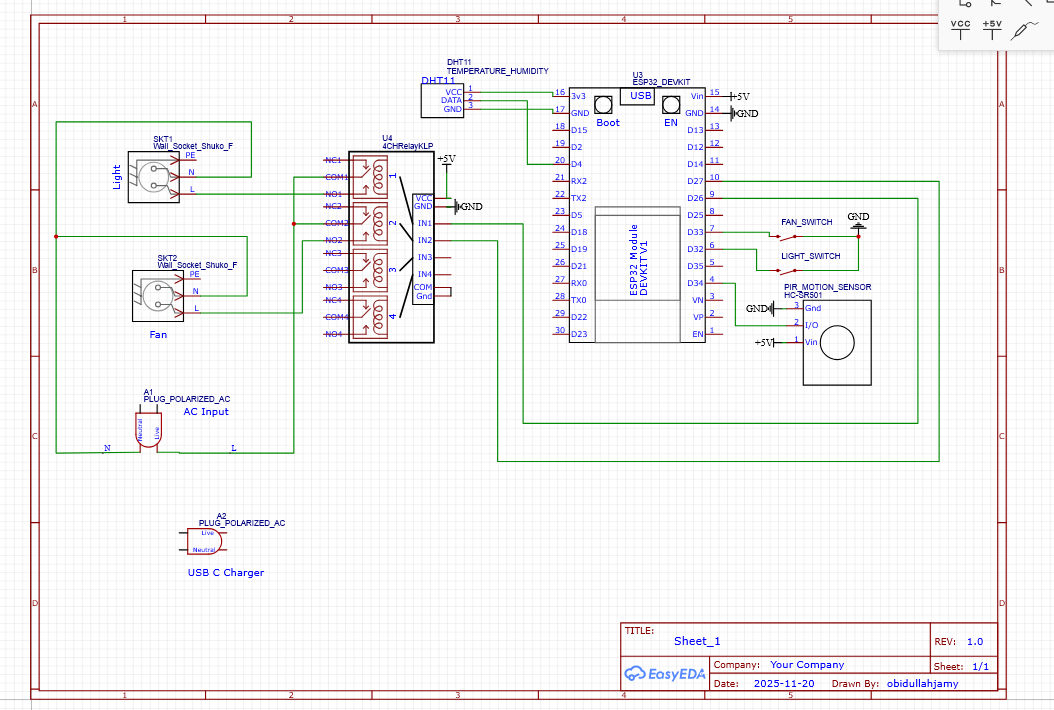
\includegraphics[width=0.95\textwidth]{circuit_diagram.jpg}
\caption{Complete Circuit Diagram - Shows AC power input (A1), USB power (A2), all connections between ESP32 and peripherals}
\label{fig:circuit_final}
\end{figure}

\begin{itemize}
\item Relay module controlled by GPIO26/27
\item Wall switches connected to GPIO32/33
\item PIR motion sensor on GPIO34
\item DHT11 sensor on GPIO4
\item All grounds connected together
\end{itemize}

\newpage
\textbf{Document Version:} 1.1 \\
\textbf{Last Updated:} December 26, 2025 \\
\textbf{For:} Arduino IoT Cloud + ESP32 Home Automation Project \\

\textbf{Note:} Place \texttt{circuit\_diagram.jpg} and \texttt{flowchart.png} in the same directory as this \texttt{.tex} file.

\end{document}